\documentclass[oupdraft]{bio}
%\usepackage[colorlinks=true, urlcolor=citecolor, linkcolor=citecolor, citecolor=citecolor]{hyperref}
% \documentclass[12pt,a4paper]{article}
\pdfoutput=1
\usepackage[utf8]{inputenc}
\usepackage[]{graphicx}
\usepackage{amsmath}
\usepackage{amssymb}
\usepackage[]{color}
\usepackage{subcaption}
% \usepackage{natbib}
\usepackage{xspace}
\usepackage{calc}
% \usepackage[noae]{Sweave}
\usepackage{algorithm}
\usepackage{algpseudocode}
\usepackage{xcolor}

% \usepackage{authblk}

\usepackage[nolists,nomarkers]{endfloat}


%\usepackage{geometry}
%\geometry{a4paper, portrait, margin=1in}
%
% New commands
%
\newcommand{\ie}{\emph{i.e.}\@\xspace}
\newcommand{\eg}{\emph{e.g.}\@\xspace}
\newcommand{\nn}{\nonumber}

\providecolor{added}{rgb}{1,0,0}
\newcommand{\added}[1]{{\color{added}{}#1}}
% \newcommand{\added}[1]{#1}   % Use after correction

% \newcommand{\mcomment}[1]{\textcolor{red}{\textbf{#1}}}

\DeclareMathOperator{\E}{\mathbb{E}}
\DeclareMathOperator{\Var}{Var}
\DeclareMathOperator{\Cov}{Cov}
\newcommand{\argmin}{\operatornamewithlimits{arg\,min}}
\newcommand{\plim}{\operatornamewithlimits{plim}}

%\usepackage[amsthm,thmmarks]{ntheorem}
% \theoremstyle{plain}
% \newtheorem{theorem}{Theorem}
%\newtheorem{definition}{Definition}
%\newtheorem{proposition}{Proposition}
\newtheorem{corollary}{\normalfont\scshape Corollary}[section]
%\newtheorem{lemma}{Lemma}
%\newtheorem{assumption}{Assumption}
%\newtheorem{example}{Example}
%\renewcommand\proofSymbol{\ensuremath{\blacksquare}}



%%% RSS specific items

%\title{Sequential rank agreement methods for comparison of ranked lists}
%\author{Claus Thorn Ekstrøm}
%\author{Thomas Alexander Gerds}
%\author{Andreas Kryger Jensen}
%\author{Kasper Brink-Jensen}
%\affil{Biostatistics, University of Copenhagen}
%\renewcommand{\topfraction}{.85}
%\renewcommand{\bottomfraction}{.7}
%\renewcommand{\textfraction}{.15}
%\renewcommand{\floatpagefraction}{.66}
%\renewcommand{\dbltopfraction}{.66}
%\renewcommand{\dblfloatpagefraction}{.66}
%\setcounter{topnumber}{9}
%\setcounter{bottomnumber}{9}
%\setcounter{totalnumber}{20}
%\setcounter{dbltopnumber}{9}


\renewcommand{\topfraction}{.85}
\renewcommand{\bottomfraction}{.7}
\renewcommand{\textfraction}{.15}
\renewcommand{\floatpagefraction}{.66}
\renewcommand{\dbltopfraction}{.66}
\renewcommand{\dblfloatpagefraction}{.66}
\setcounter{topnumber}{9}
\setcounter{bottomnumber}{9}
\setcounter{totalnumber}{20}
\setcounter{dbltopnumber}{9}


\begin{document}


\title{Sequential rank agreement methods for comparison of ranked lists}

\author{CLAUS THORN EKSTRØM$^\ast$, THOMAS ALEXANDER GERDS, ANDREAS
  KRYGER JENSEN\\[4pt]
%
\textit{%
Biostatistics, Department of Public Health,
University of Copenhagen,
Øster Farimagsgade 5 B, P.O.B. 2099,
DK-1014 Copenhagen K, Denmark}
\\[2pt]
% E-mail address for correspondence
{ekstrom@sund.ku.dk}}



% Use square brackets for numbering affiliations


% Running headers of paper:
\markboth%
% First field is the short list of authors
{C. T. Ekstrøm and others}
% Second field is the short title of the paper
{Sequential rank agreement for comparison of ranked
  lists}

\maketitle


\footnotetext{To whom correspondence should be addressed.}

\begin{abstract} { The comparison of alternative rankings of a set of
    items is a general and common task in applied
    statistics. Predictor variables are ranked according to magnitude
    of association with an outcome, prediction models rank subjects
    according to the personalized risk of an event, and genetic
    studies rank genes according to their difference in gene
    expression levels. \added{We propose a sequential rank agreement
      measure to quantify the rank agreement among two or more ordered
      lists. This measure has an intuitive interpretation, it can be
      applied to any number of lists even if some are partially
      incomplete, and it provides information about the agreement
      along the lists. The sequential rank agreement can be evaluated
      analytically or be compared graphically to a permutation based
      reference set in order to identify changes in the list
      agreements.}  The usefulness of this measure is illustrated
    using gene rankings, and using data from two Danish ovarian cancer
    studies where we assess the within and between agreement of
    different statistical classification methods.}  {rank agreement;
    incomplete ranking; order statistic; methods comparison;
    permutation}
\end{abstract}

%Key words: rank agreement, partial ranking, order
%statistic, gene rankings, methods comparison, variable selection,
%permutation

\section{Introduction}

Ranking of items or results is common in scientific research and
ranked lists occur naturally as the result of many statistical
applications. Regression methods rank predictor variables according to
magnitude of their association with an outcome, prediction models rank
subjects according to their risk of an event, and genetic studies rank
genes according to their difference in gene expression levels across
samples.  \added{Two common research questions are of interest when
  several rankings of the same items are available: 1) To what extent
  do the lists agree on the rankings and how will that change as we go
  through the lists, and 2) Is it possible to identify an optimal rank
  until which the lists agree on the items?

  A typical situation where these questions arise is in
  high-dimensional genomics studies such as genome-wide association
  studies where several analysis methods (e.g., regression methods,
  lasso, random forest) can be used identify and rank millions of gene
  variants according to their association with the outcome. The
  ranking of each gene variant may vary from method to method and a
  consensus summary of agreement of the findings is needed to
  determine which gene variants to investigate more closely in
  subsequent validation studies. To minimiize expenses it is only of
  interest to consider gene variants that have high ranking across the
  different methods.  Multiple ranked lists also appear in machine
  learning where the stability of the ranks produced by a
  ``black-box''-technique can be evaluted by bootstrapping the
  data. Assessing which items are stable (i.e., consistant rankings
  across bootstrap samples) will help to weed out possible fluke
  findings.}


In this article we introduce sequential rank agreement for measuring
agreement among ranked lists.  The general idea is to define agreement
based on the sequence of ranks from a subset of the first $d$ items in
each list. As agreement metric we adapt the limits of agreement known
from agreement between quantitative variables
\citep{alt:bland:1983} but any measure for agreement
could essentially be used. Our proposed approach allows us to compare
multiple lists simultaneously, it provides a dynamic measure of
agreement as a function of the depth in the lists, it places higher
weight on items at the top of the list, it accommodates partially
observed lists of varying lengths, and has a natural interpretation
that directly relates to the ranks.  Graphical illustration of
sequential rank agreement allows us to infer any changepoints, i.e., a
list depth where a substantial change in the agreement of the lists
occur but we also provide asymptotical and randomization-based
graphical tools to compare the observed rank agreement to the expected
agreement found in non-informative data.  In this sense our approach
is a combination and generalization of some of the ideas of
\added{\citet{iriz:etal:2005}}, \citet{Carterette2009}, and
\citet{Boulesteix2009}. \citet{Carterette2009} compares two rankings
based on the distance between them as measured by a multivariate
Gaussian distribution and the latter presents an overview of
approaches for aggregation of ranked lists including bootstrap and
leave-one-out jackknife approaches. \added{\citet{iriz:etal:2005}
  proposes a plot based on the intersection of lists which is a
  special case of our setting where the agreement metric is the
  overlap proportion}. However, simple intersection also places equal
weights on all depths of the list and therefore \citet{Fagin2003}, and
\citet{Webber2010} proposed weighted intersections which put more
emphasis on the top of the lists.  Specifically, \citet{Webber2010}
define their rank-biased overlap (RBO) by weighting with a converging
series to ensure that the top is weighted higher than the potentially
non-informative bottom of the lists.  It is possible to use the
existing methods to calculate agreement of lists until a given depth,
i.e., limited to the $d$ items of each list. However, the
interpretation may not be straightforward, especially in the case of
more than two lists, and they may not accommodate partial rankings.





% Several approaches exist to measure the ``distance'' between two
% ranked lists. Of these, Kendall's $\tau$ \citep{kendall1948} and
% Spearman’s footrule $\rho$ \citep{Spearman1910} are among the most
% well-known, but these measures do not distinguish between agreement in
% the top versus towards the bottom of the lists and they both provide a
% single measure of the overall distance. \citet{Shieh1998} proposed a
% weighted version of Kendall's $\tau$ where each pair of rankings can
% be assigned different weights, and \citet{Yilmaz2008} proposed the
% $\tau_{ap}$ which places higher emphasis on the top of the lists.
% Spearman’s footrule uses the ranks of the variables for calculation of
% the distance and the use of ranks are also employed in the $M$ measure
% of \citet{Bar-Ilan2006} where the reciprocal rank differences are used
% to calculate the similarity measure.




Very recently, \citet{hall:schi:2012} proposed a method for comparing
pairwise rankings and derived the asymptotic distribution of the
endpoint where the two ranked lists no longer are in agreement. Their
approach was based on anchoring one of the two lists and subsequently
generating a sequence of 0s and 1s depending on whether the ranks in
the second list was close to the rank from the anchored
list. \citet{samp:verd:2013} followed up on this idea for pairwise
comparison of lists but used penalties based on a truncated geometric
probability instead of a 0-1 process and they evaluated the
distribution of the endpoint of agreement by computational approaches.
The asymptotic distribution in the \citet{hall:schi:2012} paper is
based on letting the number of \emph{lists} increase to infinity which
is a situation that is only relevant in special cases, whereas the
\added{simulation-based null distribution approach of
  \citet{samp:verd:2013} does not rely on asymptotic results to
  evaluate their pairwise findings.}



The manuscript is organized as follows: The next section defines
sequential rank agreement for multiple ranked lists and discuss how to
handle incomplete lists. In section 3 we show the asymptotic
distribution of the endpoint of agreement and discuss approaches to
evaluate the results obtained from sequential rank agreement.
%infer the
%distribution in small-sample situations using computational
%methods. This enables us to make inferences about the endpoint of
%agreement even for situations where there is no actual changepoint
%present but just a gradual decline in agreement.
Finally we apply the sequential rank agreement to two Danish ovarian
cancer studies and compare our method to the method of
\citet{hall:schi:2012} in a small sample simulation study before we
discuss the findings and possible extensions. The approaches
presented are implemented in the R package \texttt{SuperRanker}  found on CRAN.
% chunk 1


\section{Methods}

Consider a set of $P$ different items $X=\{X_1,\dots,X_P\}$ and a
ranking function $R: \{X_1,\dots,X_P\}\to \{1,\dots,P\}$, such that
$R(X_p)$ is the rank of item $X_p$. The inverse mapping $R^{-1}$ gives
the item $R^{-1}(r)$ that was assigned to rank $r\in\{1,\dots,P\}$. An
ordered list is the realization of a ranking function $R$ applied to
the set of items $X$.  Panels (a) and (b) of Table~\ref{tab:example}
show a schematic example of these mappings. Thus if
$R_l^{-1}(1)=X_{34}$ then item $X_{34}$ is ranked first in list $l$
and similarly $R_l(X_{34})=1$.
% 
In all what follows we consider a fixed set of items and consider the
ranking function to be a random variable. Thus, let
$R_1(X),\dots,R_L(X)$, $L\geq2$, be a sample of $L$ independent
identically distributed draws from an unknown probability distribution
function $Q$. One aim is then to test how much $Q$ resembles the
uniform distribution which assigns probability $1/P!$ to each of the
$P!$ different possible rankings. 


The agreement among the lists regarding the rank given to an item $X_p$
can be measured by the variance across the lists
\begin{align}
  A(X_p) &= \E_Q\left[\left(R(X_p)-\E_Q R(X_p)\right)^2\right]\\
   &= \sum_{r\in\Pi} \left(r(X_p)-\E_Q R(X_p)\right)^2 Q(r),\nn
\end{align}
where $\Pi$ is the set of all permutations of $X$, $Q$ is a
probability mass function on $\Pi$, and
$\E_Q R(X_p)=\sum_{r\in\Pi} r(X_p)Q(r)$. The empirical counterpart is
\begin{align}
\widehat{A}_L(X_p) = \frac{1}{L-1}\sum_{i=1}^L (R_i(X_p) - \overline{R}_L(X_p))^2, \quad \overline{R}_L(X_p) = \frac{1}{L}\sum_{i=1}^L R_i(X_p).\label{eq:empDistance}
\end{align}
For each item, the function $\widehat{A}_L$ has an interpretation as the expected
Euclidean distance of the individual rankings from the expected
ranking over the $L$ lists, and it corresponds to the same measure
that is used to compute the limits of
agreement \citep{alt:bland:1983}.

For an integer $1\le d\le P$ we define the expected set of unique
items found by merging the first $d$ elements across the possible
lists:
\begin{align}
S(d) &= \left\{X_p; \left(\sum_{r\in\Pi} 1\left(r(X_p)\le d\right) Q(r)\right) > \added{\varepsilon}\right\}\label{eq:sumset}
\end{align}
where $1(\cdot)$ denotes the indicator function\added{, and where $\varepsilon\in[0,1)$ is a pre-specified constant that sets the minimum proportion of lists that an item must be present in before it is added to $S(d)$. When $\varepsilon=0$ then an item is included as soon as it is present in just one list.}
The empirical counterpart is the set of unique items ranked less than or
equal to $d$ in any of the $L$ lists:
\begin{equation}
\widehat{S}_{L}(d) = \left\{X_p; \left(\frac{1}{L}\sum_{l=1}^L 1\left(R_l(X_p)\le d\right)\right)>\added{\varepsilon}\right\},
\end{equation}
which is exemplified in Panel (c) of Table \ref{tab:example}.

We define the \emph{sequential rank agreement} as the weighted
expected agreement of the items found in the set $S(d)$:
\begin{equation}
\added{  \textrm{sra}(d) = \left\{\begin{array}{cl}\frac{1}{|S(d)|}\sum_{p \in S(d)}A(X_p)  & \text{when $|S(d)|>0$} \\ 0 & \text{otherwise}\end{array}  \right.}\label{def:sra}
\end{equation}
where $|S(d)|$ is the cardinality of the set $S(d)$. \added{As stated, we are only interested in sra($d$) when $|S(d)|>0$.}
The empirical counterpart when $|S(d)|>0$ is equivalently given by
\begin{equation}
  \widehat{\textrm{sra}}_L(d) = \frac{\sum_{\{p \in \widehat{S}_{L}(d)\}}(L-1)\widehat{A}_L(X_p)}{(L-1)|\widehat {S}_{L}(d)|}.\label{def:sraEst}
\end{equation}

Values of \textrm{sra} close to zero when $|S(d)|>0$ suggest that the
lists agree on the rankings while larger values suggest
disagreement. \added{If $|S(d)|=0$ then no items were sufficiently
  frequent among the observed lists and we can conclude that the lists
  do not agree above the threshold $\varepsilon$.  } The sequential rank agreement will be zero for all values of $d$
when the ranked
lists are identical.
 %position or depths $d$ down the lists.


\subsection{Interpreting and applying sequential rank agreement}
\label{sec:amfol}


The sequential rank agreement is equivalent to the pooled variance of
the items found in $S(d)$. Thus, the square root of the sequential
rank agreement measures the average of the average difference in
rankings among the lists for the items we have included until depth
$d$.

In method comparison studies the observed agreement is compared to a
pre-specified acceptable limit and we can do similarly. For easy
visualization of the rank agreement we suggest to plot
$\sqrt{\widehat{\textrm{sra}}_L(d)}$ corresponding to the pooled SD
against $d$.


As an example consider the data by \citet{Golub1999} (found in
\citet{Dudoit2002}) where 3051 gene expression values measured on 38
tumor mRNA samples were used to classify between acute lymphoblastic
leukemia (ALL) and acute myeloid leukemia (AML). Several 
analysis methods are possible for these data for example marginal unequal
variances two-sample $t$ tests, marginal logistic regression analyses,
elastic net logistic regression \citep{friedman2010regularization},
and marginal maximum information content correlations (MIC)
\citep{Reshef2011}, and we want to identify a set of genes that
consistently are most likely to be associated to leukemia.

\added{
For the first two methods, the genes were ranked according to minimum
$p$ value, for logistic regression the genes were ordered by size of
the corresponding coefficients (after standardization), and MIC was
ordered by absolute correlation which resulted in the top rankings
seen in Table~\ref{tab1}. The ranked lists appear to agree that genes
2124 and 829 are among the most interesting while the best ranked
gene from MIC, gene 378, is not found in the top 10 for two of the
other methods.




% The simplest case occurs when all $L$ lists are fully observed, \ie, when
% we observe the rank of all $P$ items for all $L$ lists. Fully
% observed ranked lists are common and arise, for example, when
% different statistical methods are applied to a dataset
% to produce lists of predictors ranked according to their importance,
% or if the same analysis method is applied to data from different
% populations.

%With fully observed lists we can plot the sequential rank agreement
%\eqref{def:sra} as a function of depth $d$. An example is seen in the top
%panels of Figure~\ref{fig:example1} where four analysis methods were
%used to rank 3051 gene expression values measured on 38 tumor mRNA
%samples in order to classify between acute lymphoblastic leukemia
%(ALL) and acute myeloid leukemia (AML)
%\citep{Golub1999}. Preprocessing of the gene expression data was done
% as described in \citet{Dudoit2002} and the four different analysis
% approaches were:


The sequential rank agreement curve (using $\varepsilon=0$ to decide
that an item should be present in just a single list before it is
included) shown in the left plot of Figure~\ref{fig:example1} show the
average distance in ranks for the genes considered among the first $d$
positions. Not surprisingly, the sequential rank agreement is better
towards the top of the lists (smaller values on the $y$ axis
corresponds to \emph{better} agreement) than towards the bottom of the
lists. Figure~\ref{fig:example1} shows a substantial deterioration in agreement (higher sra) after
depth 5. Thus, if we were to restrict attention to a small set of
predictors then our prime focus would be on the items found among the
top-5 lists from Table~\ref{tab1}). The choice of which depth until
which we think the lists agree can be chosen either from a
pre-specified threshold for an acceptable difference in rankings or
from a pre-specified item set size. A changepoint analysis on the
sequential rank agreement would be able to identify depths where a
substantial increase/change in rank agreement occurs and would be
another way to identify sets of items that share agreement among the
lists if a pre-specified acceptable rank agreement threshold is not
given.}

% latex table generated in R 3.2.3 by xtable 1.8-2 package
% Fri Apr  8 10:22:58 2016

% chunks 2,3,4,5,6,7

% If the lists agree on all items then the sequential rank agreement is
% zero for all depths. 
Generally, changes in the level of rank agreement suggest that there
are sets of items that are ranked similarly in all lists while other
items constitute set(s) with vastly different
ranks. When the lists are likely to agree on a few top ranked items
then the sequential rank agreement curve will start low and
then increase until it levels off exactly as is seen in
Figure~\ref{fig:example1}.

\subsection{Analysis of incomplete lists}
Incomplete or partial lists are a common occurrence that arise, for
example, in case of missing data (items), when comparing top $d$ list
results from publications, or when some methods only rank a subset of
the items. For example, penalized regression such as the Lasso
provides a sparse set of predictors that have non-zero
coefficients. There is no obvious ordering of the set of predictors
whose coefficient has been shrunk to zero and thus we end up with a
partial ordering.  Incomplete lists also occur if for example the analyst
restricts attention to the ranks of items that have been found to be
statistically significant.

Sequential rank agreement can be generalized to incomplete lists in
the following way. Let $\Lambda_l\subset X$ be the subset of $d_l$
items that have been ranked highest in list $l$.  The case where all
lists are incomplete at the same depth $d$ corresponds to
$d_1=\cdots=d_L=d$. For incomplete lists the rank function becomes
\begin{equation}
	\widetilde R_l(X_p) = \begin{cases}
	     \{R_l(X_p)\} & \text{for } X_p\in \Lambda_l\\
	     \{d_l+1,\dots,P\} & \text{for} X_p \not\in \Lambda_l
        \end{cases}
\end{equation}
where we only know that the rank for the unobserved items in list $l$
must be larger than the largest rank observed in that list.

The agreement, $A(X_p)$, cannot be computed directly for all
predictors in the presence of incomplete lists because the exact rank
for some items will be unknown. Also, recall that the rankings within
a single list are not independent since each rank must appear exactly
once in each list. Thus, we cannot simply assign the same number
(\eg, the mean of the unassigned ranks) to the missing items since
that would result in \emph{less} variation of the ranks and hence less
variation of the agreement, and it would artificially introduce a
(downward) bias of agreement for items that are missing in multiple
lists.

Instead we randomize the ranks $\{d_{l}+1,\dots,P\}$ to the items that
do not occur in list $\Lambda_l$. One realization of the $L$ rankings
of the set $X$ is obtained by randomizing the missing items of each
list. By randomizing a large number of times we can compute
\eqref{def:sra} for each realization, and then compute the sequential
rank agreement as the pointwise (for each depth) average of the rank
agreements. The algorithm is described in detail in
Algorithm~C in the appendix.


The proposed approach is based on two assumptions: 1) that the most
interesting items are found in the top of the lists, and 2) that the
ranks that are missing from the lists provide so little information
that it is reasonable to assume that they can be represented by a
random order. The first assumption is justifiable because we have
already accepted that it is reasonable to rank the items in the first
place. The second assumption is fair in the light of the first
assumption provided that we have a ``sufficiently large'' part of the
top of the lists available.

When the two assumptions are satisfied then it is clear that the
interesting part of the sequential rank agreement curves is restricted
to depths where the number of items without ranks available is
low.
%Generally, without additional prior knowledge about the
%underlying distribution of the ranks it seems reasonable to restrict
%attention of the sequential rank agreement to lists no longer than the
%longest of the $L$ lists examined.
Similar to fully observed lists we generally expect the sequential
rank agreement to start low and then increase unless the lists are
completely unrelated (in which case the sequential rank agreement will
be constant at a high level) or if the lists mostly agree on the
ranking (in which case the sequential rank agreement will also be
constant but at a low level). For incomplete ranked lists we also
expect a changepoint around the depth where the lists are become
incomplete. This is an artefact stemming from the fact that we assume
that the remainder of the lists can be replaced by a simple
permutation of the missing items. \added{Note that if an item is
  ranked highly in a few lists but unranked in the remaining lists
  then it gets poor rank agreement since we only compare
  whether the lists agree on their rankings and in this case they
  clearly do not.}

The right-most plot of Figure~\ref{fig:example1} shows the impact
of restricting the Golub data such that only top-20 lists are
available instead of full lists of length 3051 (20 was chosen to
resemble the list lengths that might be harvested from published manuscripts). The sequential rank agreement increases much quicker
because the incomplete lists introduce more noise in the estimation of
the agreement, but it is still possible to see that the top of the
list has a sequantial rank agreement that is not substantially
different from the full lists.



% \subsection{Comparison to average overlap}
% The average overlap is a measure that is widely used in comparisons of
% two fully observed ranked lists \citep{Fagin2003,Webber2010} and the
% idea behind the average overlap closely resembles the sequential rank
% agreement. In this section we present an extension of the average
% overlap to more that two lists and compare this to sequential rank
% agreement.

% The overlap among $L$ lists observed until depth $d$ is defined as the
% proportion of items that are found in all $L$ lists compared to the
% possible number of items found in all lists observed until depth $d$:
% \begin{align}
%   O(d) = \frac{| \cap_{l=1}^L \{R_l^{-1}(r); r\leq d \} |}{d}\label{def:overlap}
% \end{align}
% Typically the overlap is only considered for pairwise comparisons
% \citep{Bar-Ilan2006,Boulesteix2009} but formula \ref{def:overlap}
% is easily extended to the situation where $L>2$ as shown above.

% The average overlap at depth $d$ is defined as the average of the
% overlaps until depth $d$,
% \begin{equation}
% AO(d) = \frac1d\sum_{i=1}^d O(d).
% \end{equation}
% This definition directly ensures that further emphasis is put on items
% in the top of the lists since their item specific overlap contributes
% to the calculation of average overlap at higher depths.

% There are three main drawbacks of the average overlap method: First it
% is highly sensitive to single items in the top of one the lists.  The
% average overlap profile may change dramatically depending on the
% presence or absence of similar items in the beginning of the
% lists. For example, if all lists have the same item at the top then
% the average overlap attains its maximum at 1, but if just one of the
% lists differ then the overage overlap starts at its minimum of
% 0. Secondly, when the number of lists, $L$, is high then it might be
% difficult to obtain a non-zero overlap (and hence a non-zero average
% overlap) at the beginning of the lists because the overlap will be
% zero until an item is present in all $L$ lists. Finally, the average
% overlap has an interpretation in terms of moving averages of
% percentages (of $L$ sets) which is somewhat less intuitive than our
% proposed sequential rank distance.

% In the following we compare the average overlap and the sequential
% rank agreement using the analysis of the Golub data
% \citep{Golub1999}. We consider a typical application of the average
% overlap and thus restrict attention to only two gene rankings obtained
% by the $t$ tests and logistic regression. These two marginal modeling
% approaches should result in very similar gene rankings. The first two
% columns of Table~\ref{tab1} show the actual top-10 ranking of the
% predictors.

% % chunks 8,9

% \begin{figure}[htbp]
% \begin{center}
% 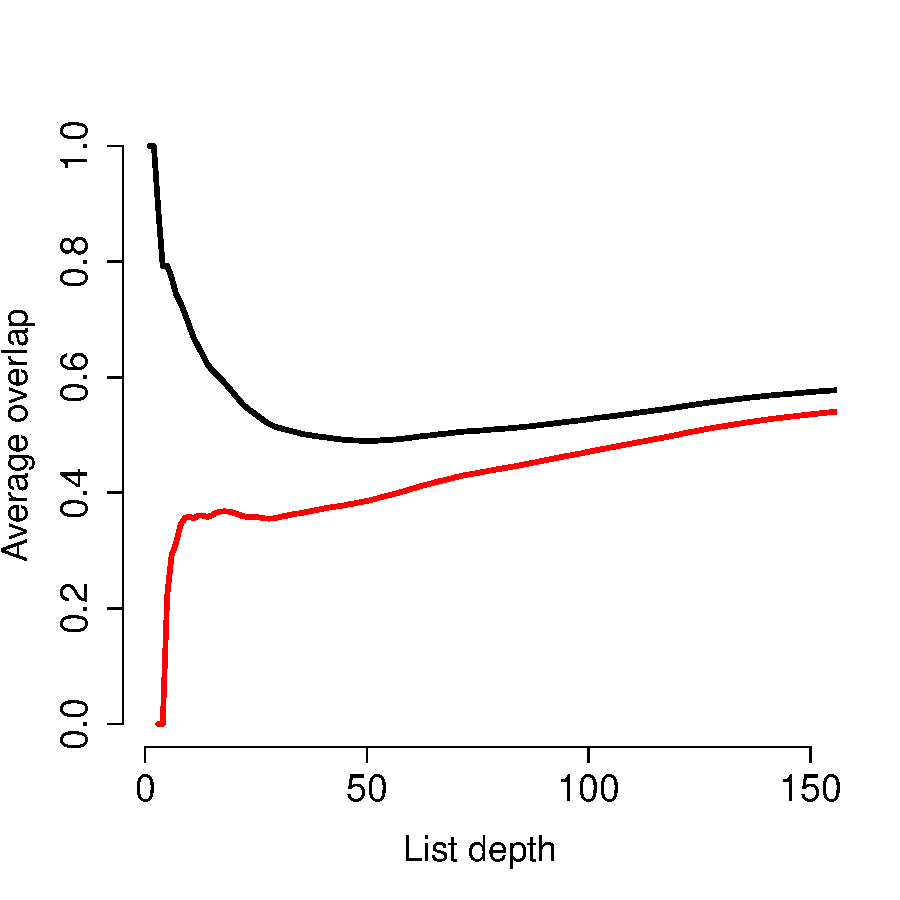
\includegraphics[width=.49\textwidth]{paper-fig-ao1}
% 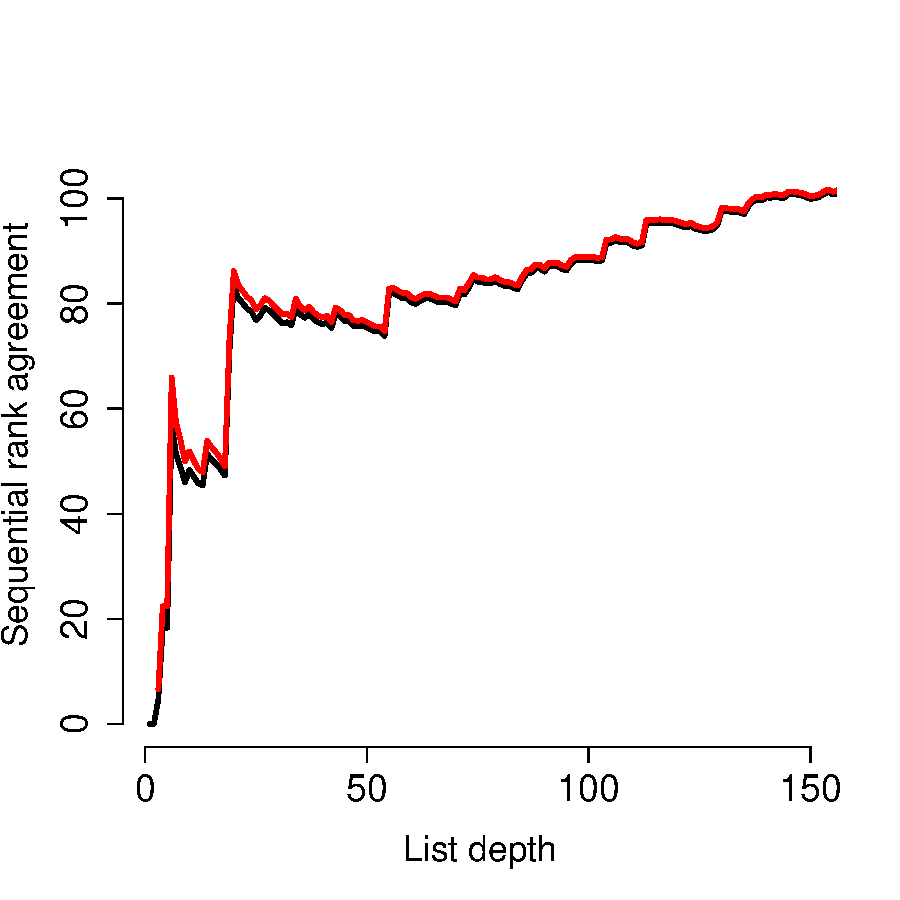
\includegraphics[width=.49\textwidth]{paper-fig-ao2}
% \end{center}
%  \caption{Average overlap (left figure) and sequential rank agreement
%  (right figure) for comparing two different analysis methods
%  (marginal $t$ test and logistic regression)
%     applied to the Golub data. The black lines are based on the full
%     set of predictors while the red lines have the two highest
%     associated predictors removed
%     from the data before computing the average overlap and sequential
%     rank agreement.}
%   \label{fig:case1}
%  \end{figure}

%  The black lines in Figure~\ref{fig:case1} show the average overlap
%  and sequential rank agreement for these data. It is clear from both
%  plots that there is perfect agreement towards the top of the ranked
%  lists: the average overlap is 1 and the sequential rank agreement is
%  zero.  However, if we remove those two items from the data (i.e.,
%  gene/predictor 2124 and 896) and redo the analyses then we get
%  substantially different curves for the average overlap but not for
%  sequential rank agreement (red lines in Figure~\ref{fig:case1}). For
%  the sequential rank agreement we get roughly the same estimate of
%  agreement from rank 3 as we did from the full dataset. This indicates
%  that sequential rank is more robust against small perturbations of
%  the data. For the average overlap the curves completely change when
%  these two items are removed and which would lead to a different
%  conclusion about the agreement among the items from rank 3 downwards.





\section{Evaluating sequential rank agreement results}
To evaluate the sequential rank agreement values we propose two
different benchmark values corresponding to two different
hypotheses. We wish to determine if we observe better agreement than
would be expected if there were no relevant information available in
the data.

The first reference hypothesis is
\begin{eqnarray}
H_0  & : &  \text{The list rankings correspond to completely randomly}\label{eq:permutationHypothesis}\\
       &  & \text{permuted lists}\nn
\end{eqnarray}
which not only assumes that there is no information in the data on
which the rankings are based but also that the methods used to provide
the rankings are completely independent.

Alternatively, we can remove the restriction of the independence among
the methods used to generate the $L$ ranked lists under the null
hypothesis that any association to the outcome is removed in the
data.


%and only require
%that there is no information contained in the rankings but that the
%rankings are all based on applying the method/approaches to the same
%data
\begin{eqnarray*}
\widetilde H_0 & :&  \text{The list rankings are based on data that contain}\\
& &   \text{no association to the outcome.}
\end{eqnarray*}

This alternative null hypothesis addresses the fact that some ranking
methods are more likely to provide similar rankings of the same data
because the ranking methods focus on the same features of the data
rather than because of any information contained in the data.


\subsection{Permutation-based inference}

$H_0$ is a quite unrealistic null hypothesis but we can easily obtain
realizations from that null hypothesis simply by permuting the items
within each list and then computing the sequential rank agreement for
the permuted lists. In the fully observed case each experiment
contains $L$ lists of random permutations of the items in $X$. For the
incomplete case we first permute the items $X_1,\dots,X_P$ and then assign missing ranks
for list $l$ from  $d_l$ to $P$ (\ie, each list has the same number of
observed rankings as was observed for list $l$ in the original
dataset). The sequential rank agreement curve from the original
lists can then be compared to, say, the pointwise 95\% quantiles of
the observed rank agreements obtained under $H_0$.

To obtain the distribution under $\widetilde H_0$ the idea is to
repeat the ranking procedures for unassociated data many times.
\added{For each resample, we
  \begin{enumerate}
  \item first permute the outcome variable in the dataset. This
    removes any association between the predictor variables and the
    outcome while keeping the structure in the predictors, and 
  \item we apply the same methods that was used for the original data to the permuted dataset to generate $L$
    new rankings and compute the sra for the unassociated data.
  \end{enumerate}
} Note that we only permute the outcomes and thus preserve the
internal structure of the predictors. This randomization approach
requires that the original data is available and as such it may not be
possible to evaluate $\widetilde H_0$ in all situations.

If the sequential rank agreement for the original data lies
substantially below the distribution of the sequential rank agreements
obtained under either $H_0$ or $\widetilde H_0$ then this suggests that
the original ranked lists agree \emph{more} than expected
in data with no information, and therefore that the information in the
lists is significantly more in agreement than what would be expected.

Figure~\ref{fig:example1} shows the empirical distributions of
sequential rank agreement under $H_0$ and $\widetilde H_0$ each based
on $400$ permutations of the Golub data from Section \ref{sec:amfol}.
\added{ Figure~\ref{fig:example1} indicates that the observed
  sequential rank agreement for the Golub data is significantly better
  than what would be expected by chance for data that contain no
  information since it lies below the reference areas if the lists
  were just random ($H_0$ corresponding to the blue area). However, if
  we consider $\widetilde H_0$ then the sequential rank agreement is
  just inside the red area and we conclude that the agreement seen in
  the Golub data is \emph{not} significantly better than what we would
  expect when we remove the association between the predictors and
  the outcome.}


The incomplete data also suggests that there may be at most 1 or 2
ranked items towards the top of the lists that yield a result better
than what would be expected (the bottom-right plot). Not surprisingly,
the sequential rank agreement under $\widetilde H_0$ is lower than the
sequential rank agreement under $H_0$ because the four methods used to
rank the data ($t$ test, logistic regression, elastic net, and MIC)
generally tend to identify the same predictors.
%even if there are only spurious associations.



\added{It is important to stress that neither $H_0$ nor
  $\widetilde H_0$ are related to questions regarding the association
  between the outcome and the predictors in the dataset. Both
  hypotheses are purely considering how the rankings agree in
  situations where the data contains no information for creating the
  rankings. It is also worth pointing out, that if the lists are short
  ($P$ low) and there are few lists ($L$ low) then the number of
  possible different permutations under the null is small and the $p$
  value obtained may be fluctuating if the number of permutations is
  small. We have found that a number of permutations over 500 works
  well even for smaller samples.}


\subsection{Asymptotic inference of change in agreement}\label{sec:chgpoint}
In many applications it is of interest to estimate a list depth which
satisfies a changepoint criterion since that corresponds to a change
in agreement among the list ranks. \added{In particular, a changepoint
  will provide a data-driven indicator as to the depth until the lists
  exhibit a change in rank agreement, and would consequently be an
  obvious choice for identifying the set of items that the lists agree
  the upon the most}. In this section we investigate the theoretical
properties of our proposed method for this specific task. As in
\citet{hall:schi:2012} we consider an infinite set of lists and study
the asymptotic behaviour for $L\to\infty$. The list lengths are not
allowed to change with $L$ since the lengths are fixed in most
applications.

We start by showing that $\widehat{\textrm{sra}}_L$ is a consistent
estimator of $\textrm{sra}$ for $L \rightarrow \infty$.
%The result is stated in Theorem \ref{thm:consistency}.

% below and requires the
% following assumptions.
% \begin{assumption}
% We assume that:
% \begin{enumerate}[label=\Alph*)]
% \item{The $L$ lists are independent and identically distributed
    % samples from a probability distribution $Q$ on the set of lists.}
% \item{$\E_Q[R(X_p)^2] < \infty$ uniformly in $p$.}
% \item{$|S(d)| > 0$ uniformly in $d$}.
% \end{enumerate}
% \end{assumption}
% We note that assumption $C$ implies that for every list depth $d$
% there must be a non-zero probability of ... under the probability
% measure $Q$.

\begin{theorem}
  Assume that $\{R_l(X)\}_{l=1}^L$ are independent draws from a
  probability distribution $Q$ on the set of lists $\Pi$. Then
  $\left\|\widehat{\textrm{sra}}_L - \textrm{sra}\right\|_\infty =
  o_P(1)$.
\label{thm:consistency}
\begin{proof}
See App. A in the supplement.%ary% material.%\ref{sec:appA}.
\end{proof}
\end{theorem}

We now define the changepoint as the first crossing point of the
sequential rank agreement and a threshold function
$q\colon\,\{1,\ldots,P\} \mapsto \mathbb{R}_{\geq 0}$. The values of
$q$ could be a deterministic constant or, % in the experimental setting,
for example, the limits-of-agreement obtained in randomly permuted
lists corresponding to the null-hypothesis in equation
(\ref{eq:permutationHypothesis}). We define the superlevel set of the
sequential rank agreement with respect to $q$ as
\begin{align}
  \mathcal{L}(q) = \left\{d : \textrm{sra}(d) \geq q(d)\right\}.
\end{align}
A changepoint $d^\ast(q)$ in the list agreement is then defined by the position
\begin{equation}
  d^\ast(q) =
  \begin{cases}
    \inf(\mathcal{L}(q)) & |\mathcal{L}(q)| > 0\\
  P & |\mathcal{L}(q)| = 0
  \end{cases}
\end{equation}
corresponding to the first list depth where the sequential rank
agreement exceeds the threshold if such a position exists. Otherwise,
the full list is in agreement according to $q$ and the changepoint is
set to the full length of the lists. The empirical superlevel set is
similarly defined as
\begin{align}
 \widehat{\mathcal{L}}_L(\widehat{q}_L) = \left\{d : \widehat{\textrm{sra}}_L(d) \geq \widehat{q}_L(d)\right\}
\end{align}
where the threshold function may depend on the sample size.
% as well.
The estimated changepoint is% therefore
\begin{align}
  \widehat{d^\ast_L}(\widehat{q}_L) &= 1(|\widehat{\mathcal{L}}_L(\widehat{q}_L)| > 0)\inf \widehat{\mathcal{L}}_L(\widehat{q}_L) + 1(|\widehat{\mathcal{L}}_L(\widehat{q}_L)| = 0)P.
\end{align}

The consistency of the estimated changepoint, $\widehat{d^\ast_L}(\widehat{q}_L)$, follows from Theorem \ref{thm:consistency} by the following corollary. 
\begin{corollary}\label{thecor}
Let $\widehat{q}_L$ be a positive threshold function such that $\left\|\widehat{q}_L - q\right\|_\infty = o_P(1)$ for some limiting
function $q$.  Then $\widehat{d^\ast_L}(\widehat{q}_L) \overset{P}{\longrightarrow} d^\ast(q)$ for $L \rightarrow \infty$.
\label{cor:consistency}
\begin{proof}
See App. B in supplement.%ary material.%\ref{sec:appB}.
\end{proof}
\end{corollary}


Corollary \ref{thecor} indicates that we can use the threshold
function $\widehat{q}_L$ estimated under the null hypothesis as
discussed in the previous section as a limiting threshold function for
inferring the depth $d$, where the observed sequential rank agreement
first crosses the threshold of the null threshold, \ie, the depth
until which the observed ranked lists are in better agreement than
expected under the null hypothesis. In that sense the threshold
function serves the same role as the limits of agreement in method
comparison studies, except that the threshold function is not constant
but can accommodate the changing nature of the number of items used
for the computation of the sequential rank agreement for a given depth.
%
In practice we can compute an estimate of the threshold function under
the null using the permutation approach sketched in the previous
section which makes it relevant even for small sample settings.

% \mcomment{Elaborate more on how to apply this in practice (finite
  % sample/bootstrap/etc.) and that $q$ is similar to LoA BA-style?  }

\section{Application to ovarian cancer data}
We now consider an application of the sequential rank agreement to two
datasets consisting of MALDI-TOF (Matrix-Assisted Laser
Desorption/Ionization Time Of Flight) mass spectra obtained from blood
samples from patients with either benign or malignant ovarian
tumors. The datasets are sub-samples of the Danish MALOVA and DACOVA
study populations.

The MALOVA study is a Danish study on ovarian cancer
\citep{Hogdall:2004:Cancer:15160342} where all Danish women diagnosed
with an ovarian tumor and referred for surgery from the participating
departments of gynecology were enrolled continuously from December
1994 to May 1999. For the purpose of illustration we use a random
sub-sample of $119$ patients with a total of $58$ patients with
malignant ovarian cancers as cases and $61$ patients with benign
ovarian tumors as controls. The DACOVA study is another
Danish study on ovarian cancer which included about
$66\%$ of the female population of Denmark
\citep{bertelsen1991protocol}. The study aimed to continuously enroll
all patients that were referred to surgery of an ovarian tumor
clinically suspected to be cancer during the period from 1984 to
1990. We use a random sub-sample from the DACOVA study of $54$
malignant ovarian cancers and $59$ benign ovarian tumors/gynecologic
disorders.

Each spectrum consists of $49642$ samples over a range of mass-to-charge ratios
between $800$ to $20000$ Dalton which we downsample on an equidistant grid of
5000 points by linear interpolation. We then preprocess the downsampled
spectra individually by first removing the slow-varying baseline intensity
with the SNIP algorithm \citep{ryan1988snip} followed by a
normalization with respect to the total ion count. Finally, we standardize
the $5000$ predictors to have column-wise zero mean and unit variance in
each dataset.

We use the two datasets to illustrate how the sequential rank
agreement can be applied in two different scenarios. In the first
scenario we assess the agreement of four different statistical
classification methods in how they rank the predictors according to
their importance for distinguishing benign and malignant tumors. In
the second scenario we assess the agreement among rankings of
individual predicted risks of having a malignant tumor. The first
scenario is relevant in the context of biomarker discovery and the
latter is important e.g., when ranking patients according to immediacy of
treatment.

Four classification methods are considered: Random Forest
\citep{breiman2001random} implemented in the R package
\texttt{randomForest} \citep{liaw2002classification}, logistic Lasso
\citep{tibshirani1996regression} and Ridge regression
\citep{segerstedt1992ordinary} both implemented in the R package
\texttt{glmnet} \citep{friedman2010regularization}, and Partial Least
Squares Discriminant Analysis (PLS-DA) \citep{boulesteix2004pls}
implemented in the R package \texttt{caret} \citep{Jed-Wing:2014aa}.
%
All four methods depend on a tuning parameter. The tuning parameter for
Lasso and Ridge regression is the degree of penalization, and for PLS-DA
it is the number of components (the dimensionality of the subspace).
We estimate these separately for each sub-sample by a 20 times repeated
5-fold cross-validation procedure. For the Random Forest we grow a fixed
number of $5000$ trees and let the tuning parameter be the number of
predictors randomly sampled at each split. We estimate this by a binary
search with respect to minimizing the Out-of-Bag classification error estimate.


In both scenarios we use the MALOVA data to train the statistical
models, and in both situations the agreements are assessed with
respect to perturbations of the training data in the following
manner. We draw 1000 random sub-samples (without replication)
consisting of 90\% of the MALOVA observations and train the four
models on each sub-sample.
%We use 1000 iterations for the sub-sampling
%procedure.


The implementation of Lasso and Ridge regression in the
\texttt{glmnet} package offers three different cross-validated
optimization criteria for the penalty parameter: total deviance,
classification accuracy and area under ROC. We apply all three
criteria to investigate their effect on the sra.
Note that these models produce incomplete lists depending on
the value of the penalty parameter.


\subsection{Agreement of predictor rankings}
For each of the four methods, each of the 1000 models trained on
the 1000 sub-samples of the MALOVA data produces a ranking of the 5000
predictors according to their importance for discriminating between
the tumor types. For the Random Forest classifier the predictors are ranked according
to the Gini index, while for the logistic Lasso and Ridge regression
models we order by absolute magnitude of the estimated
regression coefficients. For the PLS-DA model the importance of the
predictors is based on a weighted sum of the absolute coefficients
where the weights are proportional to the reduction in the sums of
squares across the components.

The top right panel of Figure \ref{fig:app1} shows the sequential rank
agreement of the estimated importance of the 5000 predictors.  For
clarity of presentation we zoom in on the agreement up to list depth
600. At deeper list depths all agreement curves are approximately constant.
%
As expected, most of the sequential rank agreement curves start low,
indicating good agreement, followed by an increase until they become
approximately constant. This has the interpretation that the
agreement across the sub-samples is higher in the top as
compared to the tail of the lists for all these classification
methods. The changepoints where the curves become approximately
constant are the list depths where the ranks of the remaining items
become close to uniformly random.

A not expected shape of the agreement curves is seen for the Ridge
models for all three tuning criteria. They all show higher
disagreement in the top of the lists followed by a decrease. The
reason behind this behavior is rather subtle. Looking at the
distribution of the absolute value of the regression coefficients we
see that a large proportion of them are numerically very close to zero
and have almost equal absolute value. This is a general feature of the
Ridge models in this dataset and seen for all the 1000 trained models.
This implies that when predictors are ranked according to the
magnitude of their coefficients, their actual order becomes more
uncertain and more close to a random permutation. This problem can be
alleviated by truncating all predictors with absolute coefficient
values below a given threshold thereby introducing an artificial
incompletion of the lists.  For the Ridge models tuned with the
deviance criterion, Figure \ref{fig:app1} (bottom left) shows the the
sequential rank agreement where for each of the 1000 trained models
the predictors were artificially censored when their absolute
coefficient value was lower than the $0.1\%$ quantile of the 5000
absolute coefficient values. The curve was calculated using Algorithm
1 from the appendix with $B=1000$ and $P=5000$. The corresponding
curve from Figure \ref{fig:app1} (top right) is shown for
comparison.  Even though the number of predictors with missing ranks is very
small compared to the total number of predictors, the effect on the
sequential rank agreement is substantial and with the artificial
censoring the shape of the curves is as expected, starting low and
then increasing. 

Looking at the agreement curves for the Lasso models in Figure
\ref{fig:app1} (top right) we clearly see the effect of the sparsity
inducing penalization giving rise to incomplete lists. These curves
were similarly calculated using the algorithm and $1000$ random
permutations. Under the deviance optimization criterion the median
number of non-zero coefficients was 33 (range 16 to 50) and for the
class accuracy criterion 14 (range 4 to 56). These values correspond
to the list depths where the agreement curves become constant as a
result of the subsequent censoring.




\subsection{Agreement of individual risk predictions}
\label{sec:airp}
To assess the stability of the individual risk predictions we apply
the predictors from the DACOVA dataset to each of the models. The
predicted probabilities are then ranked in decreasing order such that
the patients with the highest risk of a malignant tumor appears in the
top of the list. Figure \ref{fig:app1} (top left) shows the sra separately
for each method, based on the 1000 risk predictions obtained from the
models trained in the same $1000$ random sub-samples of the MALOVA
data.

Most curves start low and then increase indicating higher agreement
among high risk patients. This is expected if we rank the individuals
according to highest risk of disease. However, it is also expected
that individuals with very low risk also show high agreement. In this
case we order the patients according to (high) risk prediction but we
could essentially also have reversed the order to identify the
patients that have low risk prediction.

An exception is the risk prediction agreement for the Lasso tuned with the AUC criterion which
shows very low agreement among the high values of the predicted
risks. The reason is that optimizing the penalty parameter with
respect to the AUC criterion tends to favor a very high penalty value
causing only a single predictor to be selected in each of the 1000
iterations. This results in a lack of generalizability to the DACOVA
data which gives rise to the higher disagreement in the predicted risks.
In the extreme case where the penalty becomes so high
that none of the predictors are selected by the Lasso, the sequential
rank agreement for the predicted probabilities becomes undefined since
all the ranks will be ties.


Comparing the top left and right panels of Figure \ref{fig:app1} it can
further be seen that some of the methods show better agreement with
respect to the predicted probabilities than for ranking the importance
of the predictors and vice versa. Ridge regression shows higher agreement across training
sets for the risk predictions than PLS-DA, and PLS-DA shows higher
agreement for predictor importance than Ridge regression.

Lasso shows similar agreement for ranking the risk predictions as
PLS-DA (except for the AUC criterion), and poorer agreement for
ranking predictors. This reason for the latter is the high
auto-correlation between the intensities in the mass spectra which
leads to collinearity issues in the regression models. It is
well-known that variable selection with the Lasso does not
perform very well when the predictors are highly correlated. The
collinearity does, however, not affect the agreement of the risk
predictions (Figure \ref{fig:app1}, top left), since
the specific variable selected is not that important for 
% it is not so important which specific variable that gets selected from
a group of highly correlated predictors when the purpose is risk
predictions.

It appears that Ridge regression tuned with the AUC criterion achieves
the best performance with respect to the stability of ranking the
individual predicted risk probabilities. It must, however, be stressed
that the sequential rank agreement in this application is only
concerned with the agreement of the risk predictions across
sub-samples and not with the actual accuracy of the risk
predictions. Thus, we also computed the AUC values for the different models
based on the DACOVA data. The distributions across the $1000$
sub-samples for a selection of the models is shown in the bottom right panel
of Figure \ref{fig:app1}.  Here we see that PLS-DA attains the highest
AUC values with a median value of $0.70$ while the Ridge model with
the AUC criterion attains a median AUC of $0.49$. This implies that
while Ridge regression optimized with respect to the AUC criterion
achieves the best sequential rank agreement, it performs similar to a
random coin toss with respect to classifying the DACOVA patients.
In practice both concerns are of importance.


\section{Simulation study --- comparison of list agreements}

We present results from a simulation study where we compare the small
sample properties of the sequential rank agreement to the topK method
\citep{hall:schi:2012}.
\added{The purpose of the simulations were twofold: First we want to
  investigate the rank agreement as it changes with threshold $q$ and
  number of lists $L$. Secondly, we want to compare the results from sra with the topK for a realistic situation where
  the true, underlying agreement is not governed by a simple
  probability distribution. Thus, we are interested in two features of
  the methods: the depth until which they agree, and the number of
  unique predictors found.

  To define the depth of agreement for sra we set a constant threshold
  function to an integer $q$ and report the first crossing point,
  i.e., the smallest list depth where sra exceeds $q$ (as implemented
  in the \texttt{sra} function from our package \texttt{SuperRanker} using
  the median absolute distance argument). For topK we use the function
  \texttt{j0.multi} which is implemented in the \texttt{R} package
  \texttt{TopKLists}. Specifically, we set the tuning parameter
  \texttt{v} of \texttt{j0.multi} to the value 6 and the window
  parameter \texttt{d} to $q$ and report the output parameter
  \texttt{maxK} as the depth of agreement. Thus, to make this
  comparison we assume that the first crossing point of sra and the
  result of the topK method measure the same underlying feature. }




\added{The simulations should mimic a data analysis situation where we
  have a single dataset and where important features are identified
  (and ranked) using marginal $t$ tests.  We want to used agreement to
  understand the stability of the observed feature selection.  } In
each simulation run, we first generated an ``original'' dataset with
1000 predictors and 400 observations. The predictors were drawn
independently from a standard Gaussian distribution with variance 1
such that
$$E(y_i) = \sum_{j=1}^{15}x_{ij},$$
where $y_i$ is the $i$th response, and $x_{ij}$ is the $j$th predictor
for the $i$th measurement.

For each ``original dataset'' we obtained $L$ ranked lists of the 1000
predictors by drawing $L$ bootstrap samples (with replacement) of 400
observations and then ranking the 1000 predictors according to their
marginal $t$ test statistics. Thus, we assessed the depth of agreement
among lists that are ranked with the same statistical method on
bootstrap versions of the same dataset. We report results from two
scenarios each based on 1000 simulated datasets:
\begin{enumerate}
\item[] Scenario I: Fix the number of lists \(L=8\) and vary the threshold  $q\in\{3,4,5,6,7,8,9,10\}$.
\item[] Scenario II: Fix the threshold \(q=5\) and vary the lists, $L\in\{3,5,10,50\}$.
\end{enumerate}
In both scenarios we summarized the distribution of the estimated
depth of agreement as well as the average number of unique predictors found
in the set of predictors which is selected by the estimated depth of
agreement.
 % Asymptotic results are available for both methods as the number of
 % lists increases, so this will investigate how much the results might
 % change as $L$ increases. For a fixed constant threshold of $q_L=5$ we
 % increase the number of available lists to investigate the sensitivity
 % of the results to $L$.
  % Throughout the simulations we
  % assume a constant, prespecified threshold function, $q_L$, and try
  % different values for the constant. The approach by
  % \citet{hall:schi:2012} uses a window size parameter, $K$, to
  % represent the maximum difference in rankings before they consider an
  % item in two lists to be in agreement.  Because the standard
  % deviation --- which is used in the sequential rank agreement
  % definition of $\hat{A}_L$--- squares its differences, it tends to
  % give more weight to larger rank differences and less weight to
  % smaller differences compared to the mean absolute difference.  To
  % ease comparison between the sequential rank agreement and the
  % \citet{hall:schi:2012} approach we would like to use the same
  % threshold for both methods, and in order to do this we use the
  % median absolute deviance throughout the simulations in lieu of the
  % pooled standard deviation.
 % For all parameter combinations we ran 1000 simulations and report the
 % distribution of the estimated depth of agreement and the average
 % number of different predictors found at a given depth.
The results from Scenario I are shown in the left panel of
Figure~\ref{fig:example99}. The violin plots (with rectangular kernel)
show the distributions of the estimated depths of agreement for both
methods. As expected the depth of agreement increased when the
threshold for agreement/window increased.

\added{
We see that sra results in a substantially lower depth of agreement
than the topK method. Also the average numbers of unique predictors
(bold numbers inside the plots) \added{which ideally should be 15 to
  reflect the number of true underlying predictors} are markedly
smaller --- and close to the true value --- for sra. Even larger
differences were found when we used the Euclidean distance instead of
the median absolute distance for the sequential rank agreement
(results not shown).  The right panel of Figure~\ref{fig:example99}
shows the results from Scenario II. The number of lists has little
impact on the results, and again the sra is more conservative than
topK and as a consequence sra includes fewer predictors in the
selected set where the lists agree. The effect sizes of the 15 predictors in the model is the
same and in practice we observe that the majority of the 15 predictors
are generally picked in each sample but that their individual rankings
vary substantially in the top 15 within each bootstrap sample. If the
number of influential predictors is lessened then the variance in
depth estimation and number of predictors is reduced.}
 
\section{Discussion}
In this article we address the problem of comparing ranked lists of
the same items. Our proposed method can handle both the situation
where the underlying data to generate the ranked lists are available
and the situation where the only available data is the actual ranked
lists. In addition, incomplete ranked lists where only the ranks of the
top $k$ ranked items are known can be accommodated as well. The
proposed agreement measure can be interpreted as the average distance
between an item's rank and the average rank assigned to that item
across lists.

The sequential rank agreement can be used to determine the depth at
which the rank agreement becomes too large to be desirable based on
prior requirements or acceptable differences, or it can be used to
visually determine when the change in agreement becomes too large.  In
that regard the investigator can have prior limits on the level of
agreement that is acceptable.

We have shown that sra is very versatile: it can be used not only to
compare ranked lists of items produced from different
samples/populations but that it also can be used to study the ranks
obtained from different analysis methods on the same data, and to
evaluate the stability of the ranks by bootstrapping (or sub-sampling)
the data repeatedly and comparing the ranks obtained from training the
models on the bootstrapped data.

While the sequential rank agreement is primarily an exploratory tool
we have suggested two null hypotheses that can be used to evaluate the
sequential rank agreement obtained. Note that none of the two null
hypotheses are concerned with the actual ``true ranking'' but are
purely concerned with consistency/stability of the rankings among the
lists, and consequently we cannot determine if the rankings are good but only
whether they agree. The sequential rank agreement curve can be
compared visually to the curves obtained under either of the null
distributions and point-wise $p$-values can be obtained for
each depth by counting the number of sequential rank agreements under
the null hypothesis that is less than or equal to the observed rank
agreement.
% Two simple extensions can be pursued to make more formal
% uniform tests: one would be to use a Kolmogorov-Smirnov-like test and
% use the largest difference between the variance-weighted sequential
% rank agreement curve and the mean null rank agreement curve as a test
% statistic. Alternatively, a changepoint analysis could be made on the
% sequential rank agreement in order to determine the depths at which
% there are ``jumps'' in the rank agreement. These jumps would
% correspond to depths for which the agreement among the lists was
% substantially worse and could serve as indicators for when the lists
% no longer agree sufficiently satisfactory.

Finally, we have --- whenever possible --- used all available ranks
from the lists.  We could choose to restrict attention to the rank of
items which show evidence for significance in their models. That
ensures that less emphasis is put on the agreement of the
non-significant items and it would be easier to identify a change in
agreement among the items that were deemed to be relevant.  Artificial
censoring was successfully introduced in the ridge regression
application.
%In our
%application section we have successfully introduced such an artificial
%censoring for the predictor rankings obtained with ridge regression.

We note that the sequential rank agreement is still marred by problems
that generally apply to ranking of items and/or
individuals. Collinearity in particular can be a huge problem when
bootstrapping data or when comparing different analysis methods. For
example, marginal analyses where each item is analyzed separately will
assign similar ranks to two highly correlated predictors while methods
that provide a sparse solution such as the Lasso will just rank a
single of the two predictors high.  Thus in such a scenario we would
expect low agreement of the rankings from Lasso and marginal analyses
simply because of the way correlated predictors are handled. This is
general problem for ranked lists and not a shortcoming of the
sequential rank agreement. %but is a problem
%general to all ranked lists.

Another caveat with the way the sequential rank agreement is defined
is the use of the standard deviation to measure agreement. The
standard deviation is an integral part of the limits-of-agreement as
discussed by \citet{alt:bland:1983} which is why we have followed the
analogous path. However, the standard deviation is unstable
when the number of observations is low and alternatives such
as the median absolute deviance may prove more stable in some
situations.

In conclusion we have introduced a method for evaluation of ranked
(partial/censored) lists that can be easily interpreted and that can
be applied to a large number of situations.  The method presented here
can be adapted further by using it to compare and classify statistical
analysis methods that agree on the rankings they provide or by using
the rank agreement to optimize a hyper-parameter in, say, elastic net
regularized regression where the rank agreement is used to determine
the mixing proportion between the $L_1$ and the $L_2$ penalty.
\added{Finally, the proposed method may be adapted (with some
  additional assumptions) to the situation where there are put equal
  emphasis on both ends of the lists and not just on the top of the
  lists.}
%Finally, the proposed method may be adapted (with some additional
%assumptions) to the situation where the lists are subsets of each
%other.
%We will be investigating these extensions further in the future.

\section{Supplementary Materials}
\label{sec5}

The reader is referred to the on-line Supplementary Materials for
technical appendices and proofs.


%  \appendix

% \newpage
% \section{Proof of Theorem \ref{thm:consistency}}
% \label{sec:appA}

% We start by defining the following cadlag function
% \begin{align}
%   N(p; d) = \sum_{s=1}^p 1\left(Q(R(X_s) \leq d) > 0\right), \quad p = 1,\ldots, P
% \end{align}
% which runs through the list elements in an arbitrary order and counts
% how many list elements that have a strictly positive probability to have
% rank less than or equal to $d$ under the probability measure $Q$.
% Note that the cardinality of the set $S(d)$ in equation
% (\ref{eq:sumset}) is equal to the counting process evaluated at the last element: $|S(d)| = N(P;d)$.
% The empirical counterpart of the counting process is given by
% \begin{align}
%   \widehat{N}_L(p; d) &= \sum_{s=1}^p 1\left( \frac{1}{L} \sum_{l=1}^L 1(R_l(X_s) \leq d) > 0\right)\\
%         &= \sum_{s=1}^p 1\left(\widehat{Q}_L(R(X_s) \leq d) > 0\right)\nn.
% \end{align}
% The joint law of the sequence
% $\{\widehat{N}_L(p;d)\}_{1\leq p \leq P}$ is completely determined by
% the finite set of the jump times of $N(p;d)$. Since
% $\{1(R_l(X_s) \leq d); l=1,\dots, L\}$ consists of independent and
% identically Bernoulli distributed variables with expectation
% $Q(R(X_s) \leq d)$ and finite variance it follows from the law of large numbers that
% $\widehat{Q}_L(R(X_p) \leq d) \overset{P}{\longrightarrow} Q(R(X_p)
% \leq d)$ for every $p$ and $d$ as $L \rightarrow \infty$. 
% Therefore, we have
% \begin{align}
%   \sup_{d \in 1,\ldots,P}\sup_{p \in 1,\ldots, P} \left|\widehat{N}_L(p; d) - N(p; d)\right| = o_P(1).\label{eq:countingConv}
% \end{align}

% The sequential rank agreement given in equation
% (\ref{def:sra}) may therefore be rewritten as the following integral
% with respect to $N$
% \begin{align}
%   \textrm{sra}(d) = \int_{1}^P \frac{A(X_p)}{N(P; d)}\mathrm dN(p; d).
% \end{align}
% The empirical sequential rank agreement is similarly given by
% \begin{align}
%   \widehat{\textrm{sra}}_L(d) &= \int_1^P \frac{\widehat{A}_L(X_p)}{\widehat{N}_L(P; d)}\mathrm d \widehat{N}_L(p; d) 
% \end{align}
% and it follows that
% \begin{align}
%   \sup_{d \in 1,\ldots,P}\left|\widehat{\textrm{sra}}_L(d) - \textrm{sra}(d)\right| \leq \sup_{d \in 1,\ldots,P}\left|U_L(d)\right| - \sup_{d \in 1,\ldots,P}\left|V_L(d)\right|
% \end{align}
% where
% \begin{align}
%   U_L(d) &= \int_1^P\frac{A(X_p)}{N(P;d)} \mathrm d\left(\widehat{N}_L(p; d) - N(p; d)\right)\\
%   V_L(d) &=  \int_1^P \left(\frac{\widehat{A}_L(X_p)}{\widehat{N}_L(P; d)} - \frac{A(X_p)}{N(P;d)}\right)\mathrm d\widehat{N}_L(p; d)
% \end{align}
% The conclusion of the proof therefore follows if each of these two
% terms are uniformly of order $o_P(1)$ in $d$.  For the first term we
% have that
% \begin{align}
%   \left|U_L(d)\right| \leq \left(\sup_{p \in 1,\ldots,P}\left|\frac{A(X_p)}{N(P;d)}\right|\right)\left(\widehat{N}_L(p; d) - N(p; d)\right)\biggr\rvert_1^P
% \end{align}
% where the second factor is $o_P(1)$ uniformly in $d$ by equation
% (\ref{eq:countingConv}). The first factor is $O(1)$ since $N(P;d)>0$
% uniformly in $d$ and because $A(X_p) = O(P^2)$ uniformly in $p$ by the Cauchy-Schwarz inequality. It
% thus follows that $\left|U_L(d)\right| = o_P(1)$ uniformly in $d$.

% Similarly we derive an upper bound for $V_L(d)$ by
% \begin{align}
%  V_L(d) &\leq \sup_{p \in 1,\ldots,P}\left|\frac{\widehat{A}_L(X_p)}{\widehat{N}_L(P; d)} - \frac{A(X_p)}{N(P;d)}\right| \int_1^P \left|\mathrm d\widehat{N}_L(p; d)\right|\label{eq:secondTerm}
% \end{align}
% and it follows directly from the law of large numbers that
% $\widehat{A_L}(X_p) = A(X_p) + o_P(1)$ uniformly in $p$ since
% $R_i(X_p)$ in equation (\ref{eq:empDistance}) for $i=1,\ldots,L$ are
% independent and $Q$-identically distributed random variables with
% finite second moment. Again, $\widehat{N}_L(P; d) = N(P;d) + o_P(1)$ uniformly in $d$ by equation
% (\ref{eq:countingConv}) and $N(P;d)>0$ so by the continuous mapping theorem the first factor
% in equation (\ref{eq:secondTerm}) is of order $o_P(1)$ uniformly in
% $p$ and $d$. The result then follows by noting that the second factor
% is bounded by $P$ uniformly in $d$. 




% \section{Proof of Corollary \ref{cor:consistency}}
% \label{sec:appB}
% Recall that $\mathcal{L}$ is the superlevel set of list positions
% where the sequential rank agreement exceeds the threshold function
% $q$. Let $A \triangle B = (A \setminus B) \cup (B \setminus A)$ be the
% symmetric difference between sets $A$ and $B$. It is then sufficient
% to show that $\widehat{\mathcal{L}}_L(\widehat{q}_L) \triangle \mathcal{L}(q) \overset{P}{\longrightarrow} \emptyset$
% for $L \rightarrow \infty$ where $\emptyset$ denotes the empty set.
% We have that
% \begin{align}
%   \plim_{L \rightarrow \infty}\left(\widehat{\mathcal{L}}_L(\widehat{q}_L) \triangle \mathcal{L}(q)\right) &=   \left(\plim_{L \rightarrow \infty}\widehat{\mathcal{L}}_L(\widehat{q}_L)\right) \triangle \mathcal{L}(q)\\
%   &= \left\{d : \plim_{L\rightarrow \infty} \left(\widehat{\textrm{sra}}_L(d) - \widehat{q}_L(d)\right)\geq 0\right\} \triangle \mathcal{L}(q)\nn\\
%   &= \left\{d : \textrm{sra}(d) - q(d) \geq 0\right\}\triangle \mathcal{L}(q)\nn\\
%   &= \mathcal{L}(q)\triangle \mathcal{L}(q)\nn\\
%   &= \emptyset\nn
% \end{align}
% as a consequence of Theorem \ref{thm:consistency}, the assumption that $\left\|\widehat{q}_L - q\right\|_\infty = o_P(1)$ and the continuous mapping theorem. This completes the proof.

%\bibliographystyle{rss}
\bibliographystyle{biorefs}
\bibliography{paperref}




\begin{figure}[htbp]
   \begin{center}
 \includegraphics[width=.49\textwidth]{newfig1a}
 \includegraphics[width=.49\textwidth]{newfig1b}
% 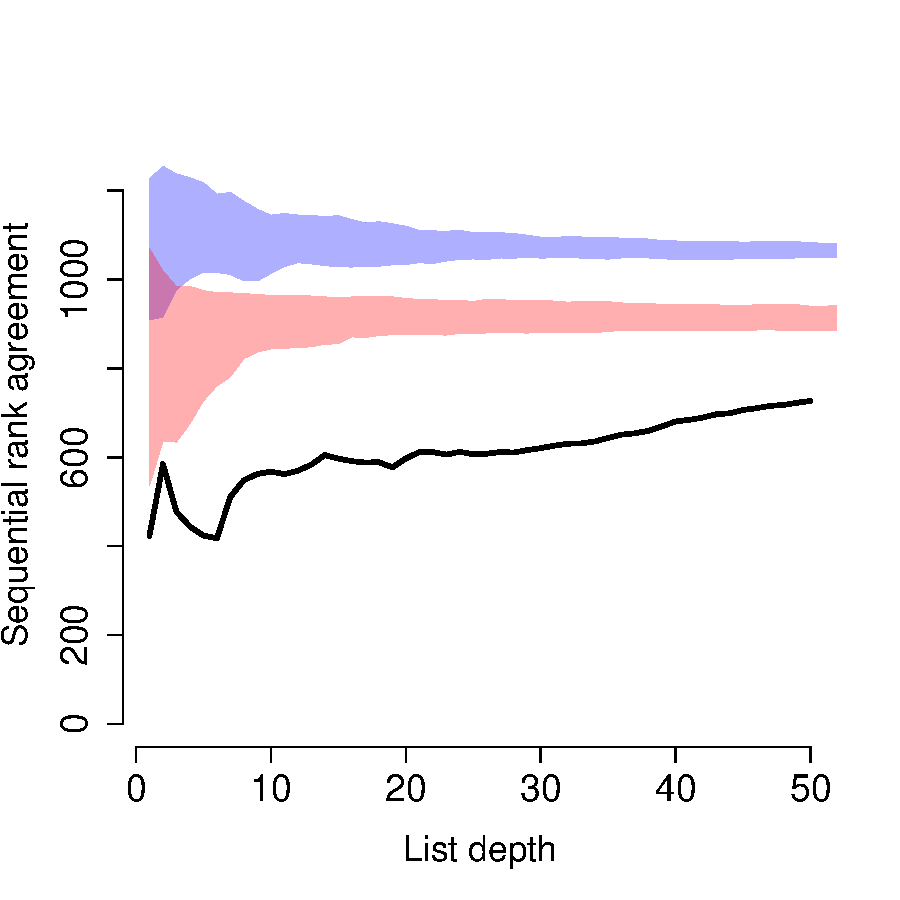
\includegraphics[width=.49\textwidth]{paper-fig1b}
% 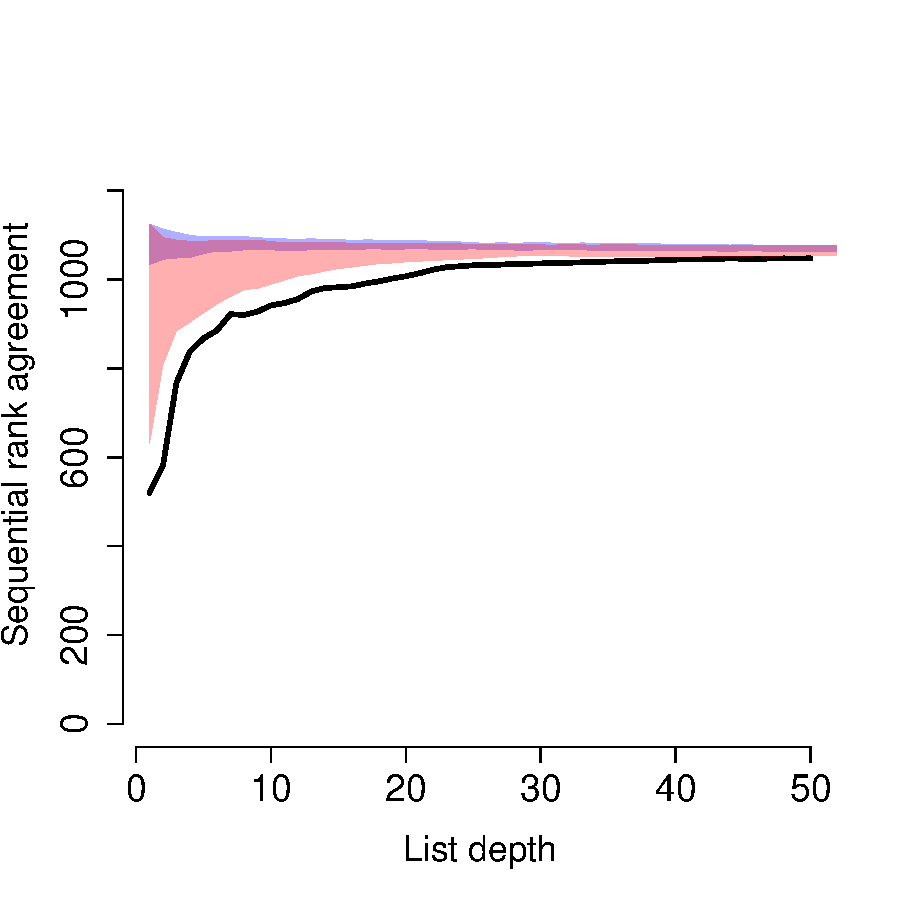
\includegraphics[width=.49\textwidth]{paper-fig2b} 
 \end{center}
 \caption{Left panel: Sequential rank agreement for 4 different
   analysis methods applied to the 3051 genes in the Golub data (black
   line). Right panel: Corresponding sequential rank agreement for the
   same data but where only the top 20 ranked items are available and
   the rank of the remaining items are not available. The blue and red
   areas correspond to the independent and randomized reference
   hypothesis areas, respectively. Note that both the $x$ and $y$ axes
   are shown on the log scale to ``zoom in'' on the top of the lists.}
 \label{fig:example1}
 \end{figure}

\newpage


\begin{figure}[htbp]
\begin{center}
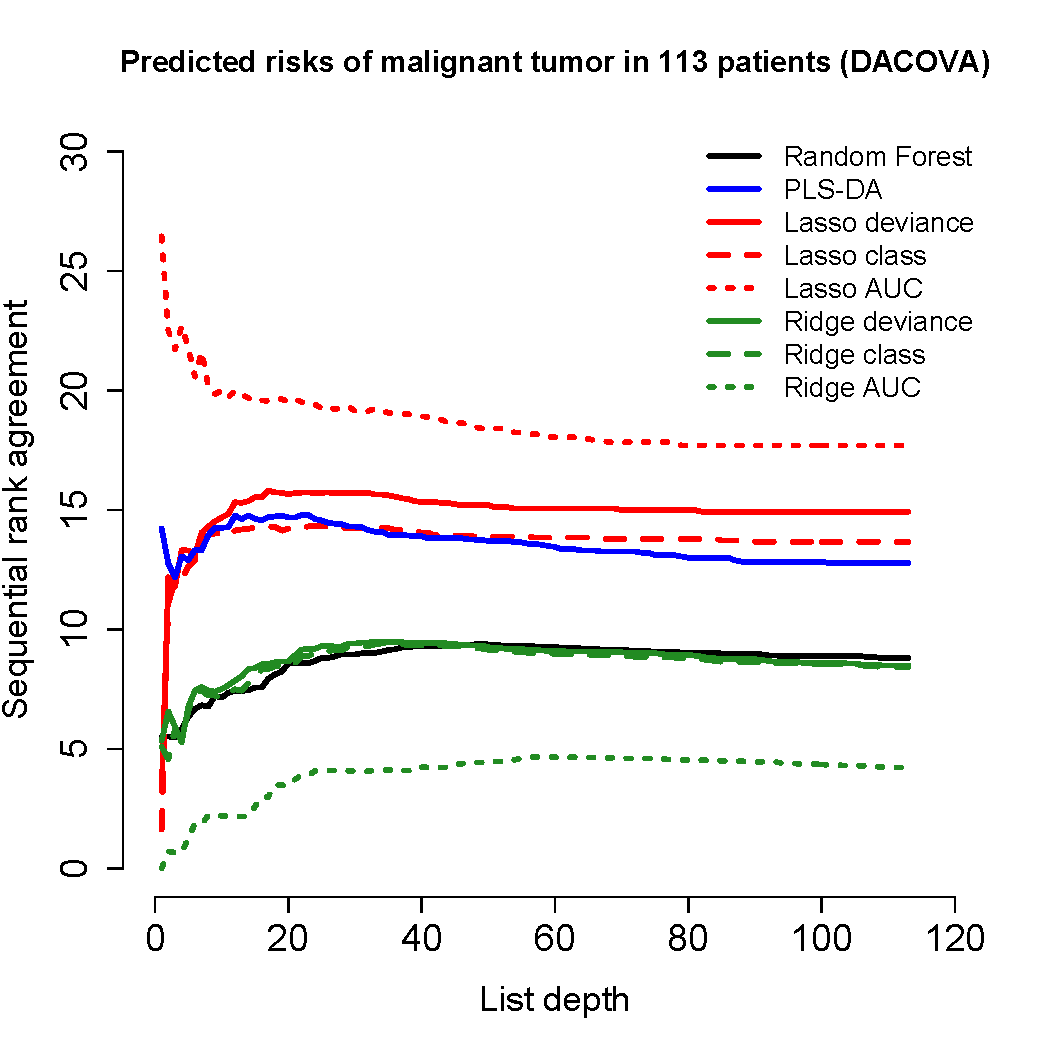
\includegraphics[width=.49\textwidth]{pics/riskAgreementPlot}%
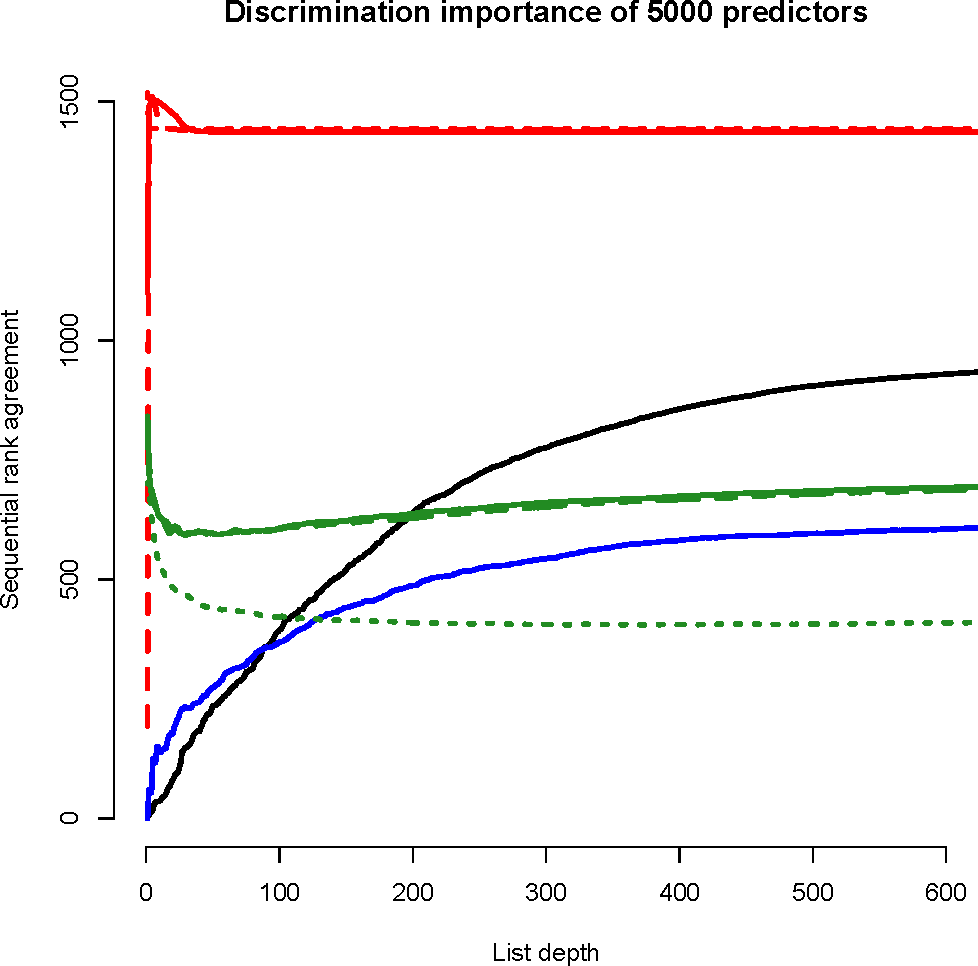
\includegraphics[width=.49\textwidth]{pics/predictorAgreementPlot}
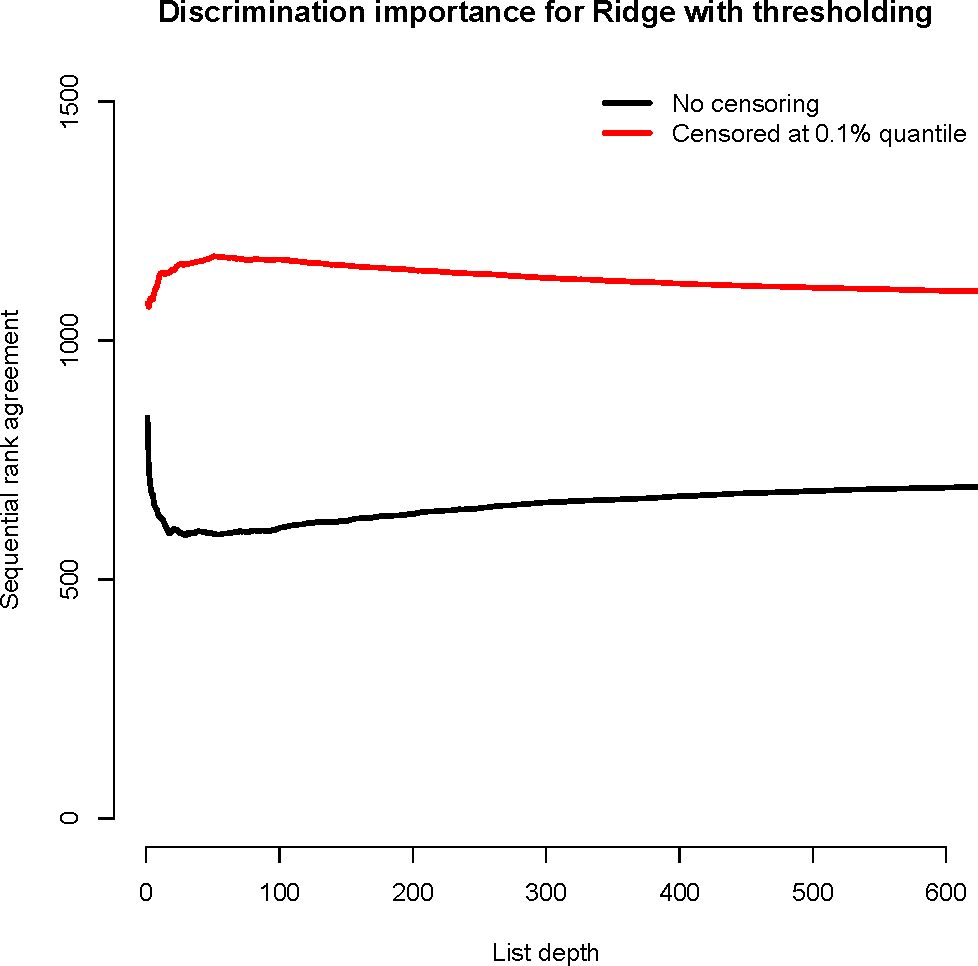
\includegraphics[width=.49\textwidth]{pics/ridgeCensoring}%
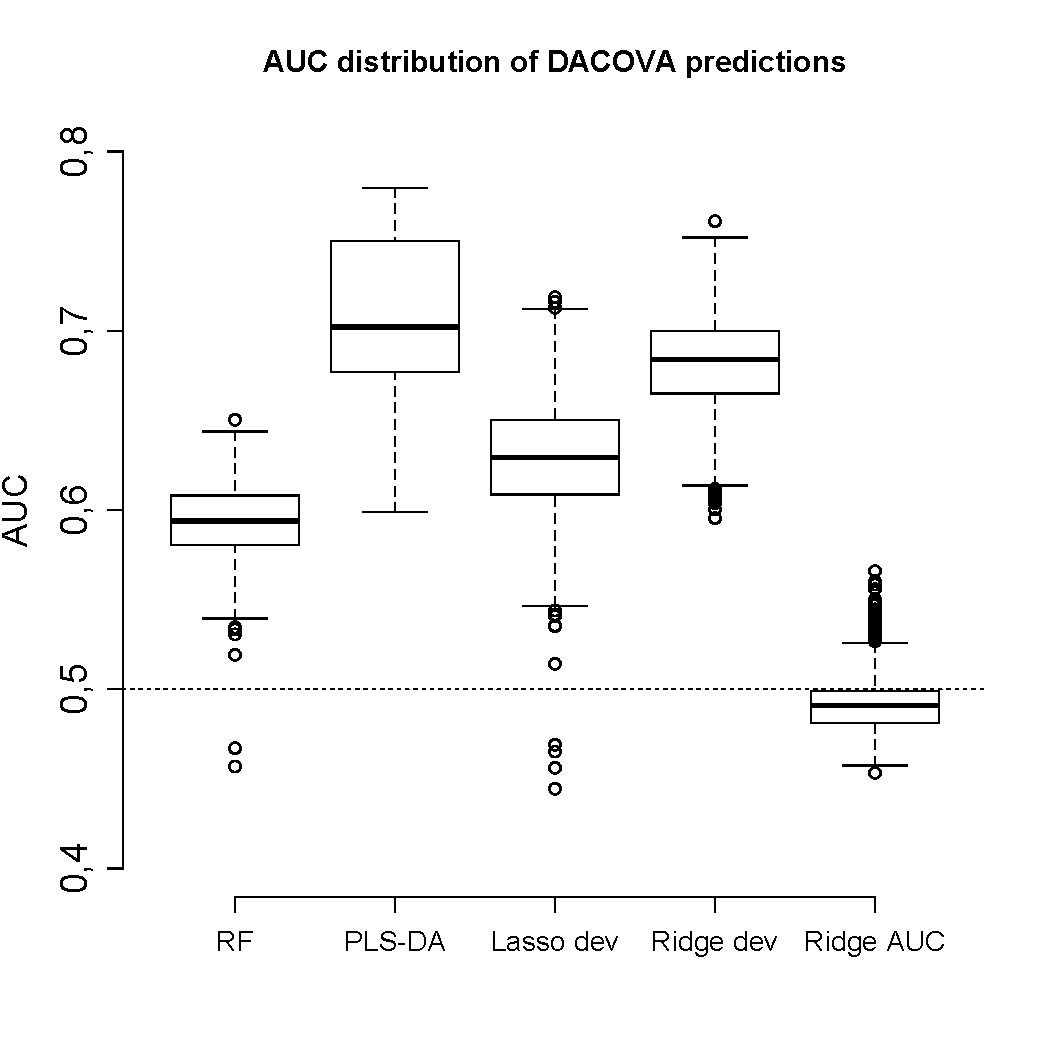
\includegraphics[width=.49\textwidth]{pics/aucPlot}
\end{center}
\caption{Top left panel: Sequential rank agreement of 1000 rankings of the
  predicted risks of malignant tumor. For each method the different
  rankings were obtained by first training models in 1000 random
  sub-samples of the MALOVA data and then predicting the risk of
  malignant tumor in the 113 DACOVA patients. Top right panel: Sequential
  rank agreement of 1000 rankings of the 5000 predictors. The rankings
  were obtained from the same 1000 trained models.
Bottom left panel: Sequential rank agreement for Ridge regression
  obtained by artificially censoring predictor ranks when their absolute
  coefficient values are lower than the 0.1\% quantile. Bottom right panel:
  Box plots of AUC values across the $1000$ sub-samples with respect
  to the known class labels of the DACOVA data.
}
 \label{fig:app1}
\end{figure}

%\newpage
%
%\begin{figure}[htbp]
%\begin{center}
%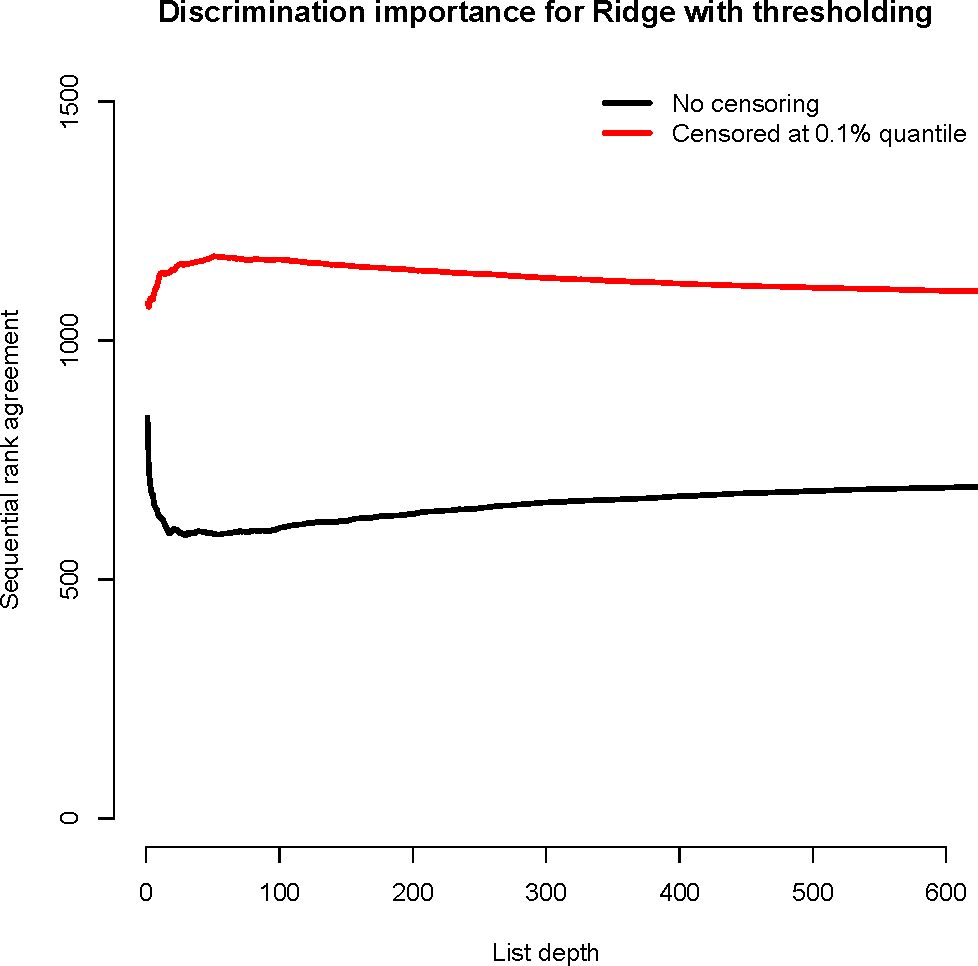
\includegraphics[width=.49\textwidth]{pics/ridgeCensoring}%
%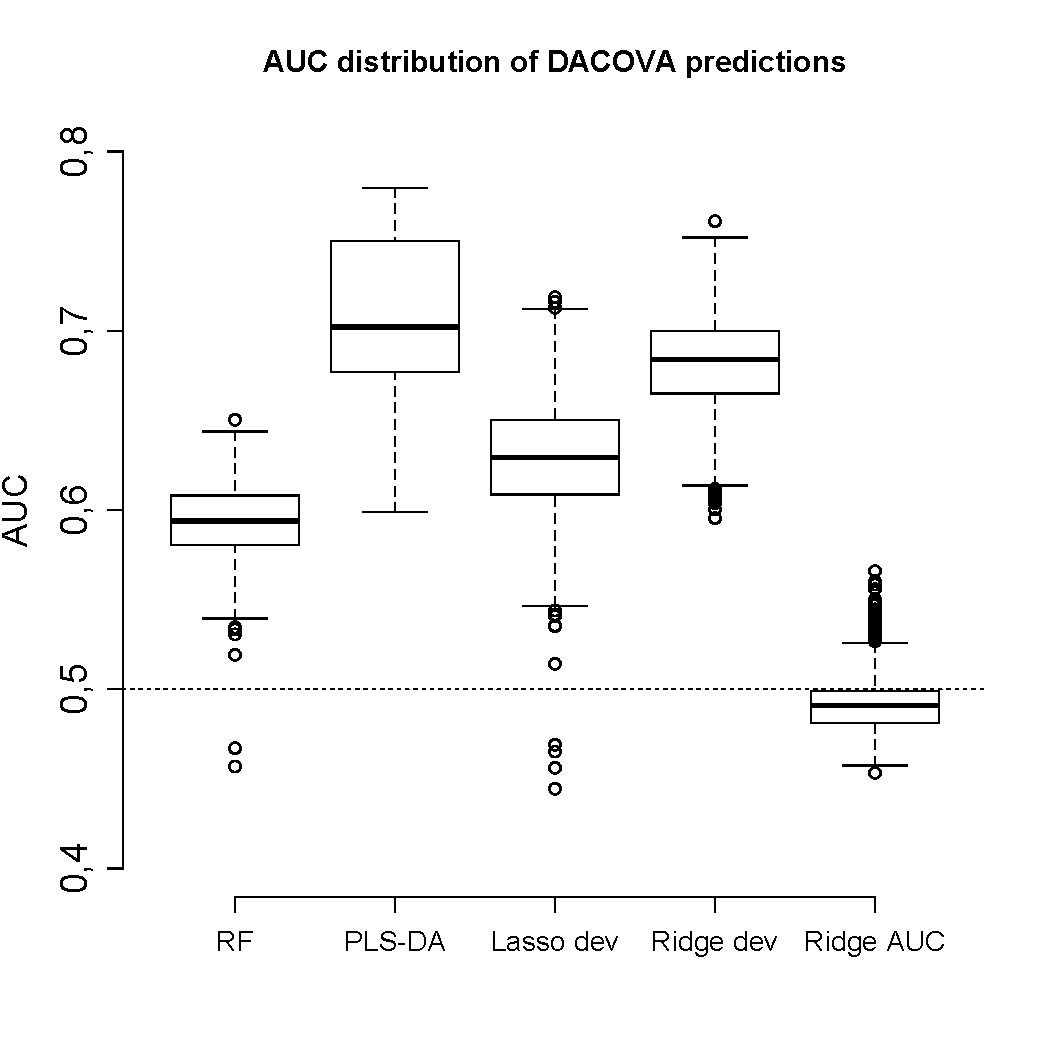
\includegraphics[width=.49\textwidth]{pics/aucPlot}
%\end{center}
%\caption{Left panel: Sequential rank agreement for Ridge regression
%  obtained by artificially censoring predictor ranks when their absolute
%  coefficient values are lower than the 0.1\% quantile. Right panel:
%  Box plots of AUC values across the $1000$ sub-samples with respect
%  to the known class labels of the DACOVA data.}
% \label{fig:app2}
%\end{figure}

\newpage


\begin{figure}[htbp]
   \begin{center}
 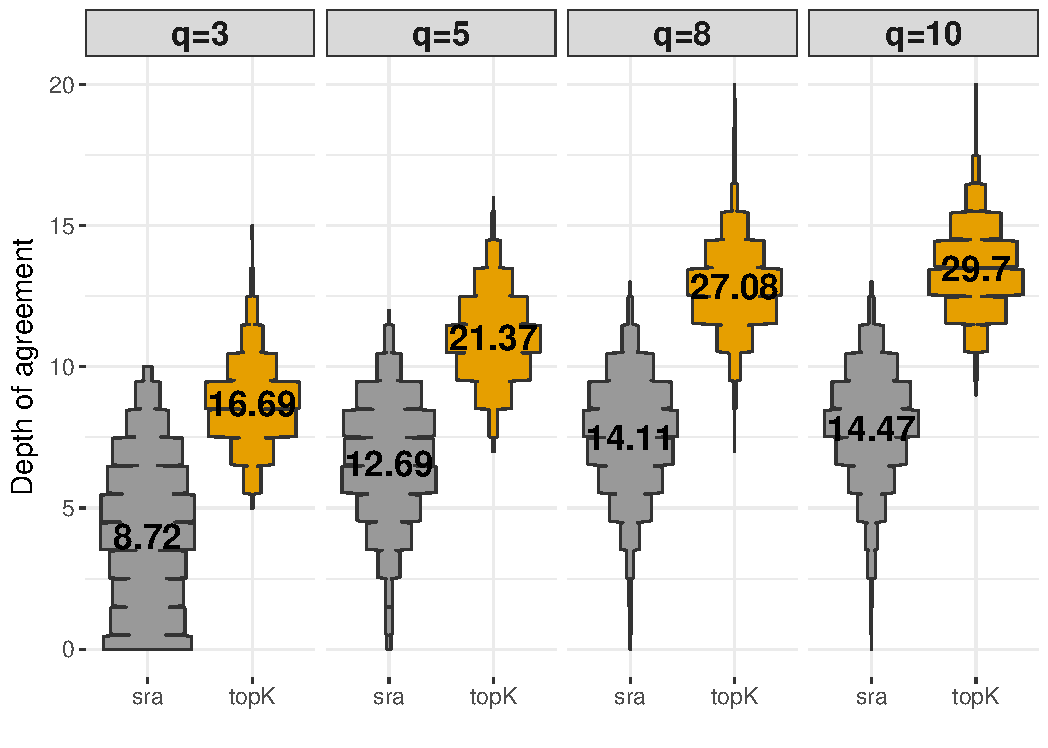
\includegraphics[width=.49\textwidth]{Ksim.pdf}
 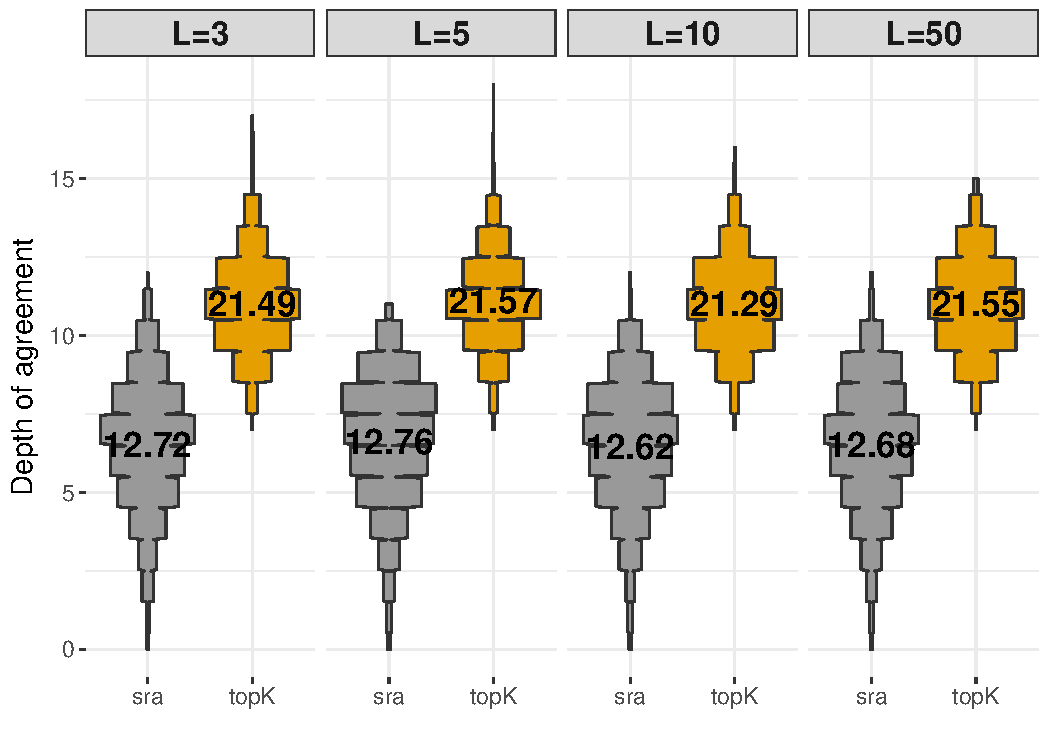
\includegraphics[width=.49\textwidth]{Lsim}
 \end{center}
 \caption{Left panel: Simulation study showing distribution of
   estimated rank agreements for sra and topK for varying thresholds
   and fixed number of lists $L=8$. The bold numbers are the average
   number of unique predictors included in the set where the lists
   agree. Right panel: Simulation results for varying number of lists
   and with fixed threshold of $q=5$.}
 \label{fig:example99}
\end{figure}




\newpage


\begin{table}[tb]
  \caption{Example set of ranked lists. (a) shows the ranked lists of
    items for each of three lists, (b) presents the ranks obtained by
    each item in each of the three lists and (c) shows the cumulative
    set of items up to a given depth in the three lists when $\varepsilon=0$ (i.e., an item is added to $S(d)$ whenever it appears in at least one list).}
\begin{center}
\footnotesize{
  \begin{subtable}{4.5cm}%
    \caption{}
      \begin{tabular}{cccc}
        \hline\hline % & \multicolumn{3}{c}{List} \\
        Rank & $R^{-1}_1$ & $R^{-1}_2$ & $R^{-1}_3$ \\ \hline
        1 & A & A & B \\
        2 & B & C & A \\
        3 & C & D & E \\
        4 & D & B & C \\
        5 & E & E & D \\ \hline
    \end{tabular}
  \end{subtable}
% \hfill
\hspace{1em}
%%%
  \begin{subtable}{4cm}%
    \caption{}
    \begin{tabular}{cccc} \hline\hline
  % & \multicolumn{3}{c}{List} \\
    Item & $R_1$ & $R_2$ & $R_3$ \\ \hline
    A & 1 & 1 & 2 \\
    B & 2 & 4 & 1 \\
    C & 3 & 2 & 4 \\
    D & 4 & 3 & 5 \\
    E & 5 & 5 & 3 \\ \hline
  \end{tabular}
\end{subtable}
% \hfill
\hspace{1em}
%%%
\begin{subtable}{4cm}%
  \caption{}
\begin{tabular}{cc} \hline\hline
% Depth   &     \\
Depth  &  $S_d$ \\ \hline
1 & $\{$A, B$\}$\\
2 & $\{$A, B, C$\}$ \\
3 & $\{$A, B, C, D, E$\}$ \\
4 & $\{$A, B, C, D, E$\}$ \\
5 & $\{$A, B, C, D, E$\}$ \\ \hline
\end{tabular}
\end{subtable}
}
\end{center}
\label{tab:example}
\end{table}

\newpage

\begin{table}[tb]
\centering
\caption{List of ranked results from the Golub data. Numbers indicate
  the predictor/gene for the given ranking and method. Only the top 10
  ranks are shown in the table. The ranked lists appear to agree that
  genes 2124 and 829 are among the most interesting while the highest
  ranked gene from MIC, gene 378, is not found in the top 10 for two
  of the other methods.}
\label{tab1}
\begin{tabular}{rrrrr}
  \hline
Ranking & Welsh's $t$ & LogReg & ElasticNet & MIC \\ 
  \hline
1 & 2124 & 2124 & 829 & 378 \\ 
  2 & 896 & 896 & 2198 & 829 \\ 
  3 & 2600 & 829 & 2124 & 896 \\ 
  4 & 766 & 394 & 808 & 1037 \\ 
  5 & 829 & 766 & 1665 & 2124 \\ 
  6 & 2851 & 2670 & 1920 & 808 \\ 
  7 & 703 & 2939 & 1389 & 108 \\ 
  8 & 2386 & 2386 & 1767 & 515 \\ 
  9 & 2645 & 1834 & 1042 & 2670 \\ 
  10 & 2002 & 378 & 2600 & 2600 \\ 
   \hline
\end{tabular}
\end{table}



\end{document}

